\documentclass[11pt]{article}

% --- Compile with: latexmk -xelatex report.tex ---
\usepackage{fontspec}
\setmainfont{Latin Modern Roman}
\usepackage{geometry}
\geometry{a4paper, margin=1in}
\usepackage{microtype}
\usepackage{booktabs}
\usepackage{tabularx}
\usepackage{array}
\usepackage{amsmath}
\usepackage{graphicx}
\usepackage{enumitem}
\setlist{nosep, leftmargin=1.4em}
\usepackage{xcolor}
\usepackage[colorlinks=true, linkcolor=black, citecolor=blue!55!black,
            urlcolor=blue!55!black]{hyperref}
\usepackage[backend=biber, style=numeric-comp, sorting=none, url=true,
            doi=false, isbn=false]{biblatex}
\addbibresource{../proposal/references.bib}
\usepackage{titlesec}
\titleformat{\section}{\large\bfseries}{\thesection}{0.6em}{}
\titleformat{\subsection}{\normalsize\bfseries}{\thesubsection}{0.6em}{}
\titlespacing*{\section}{0pt}{1.1em}{0.5em}
\titlespacing*{\subsection}{0pt}{0.8em}{0.35em}

\newcolumntype{Y}{>{\raggedright\arraybackslash}X}
\setlength{\emergencystretch}{3em}

\title{\vspace{-2.2em}\textbf{Content Disarm and Reconstruction as an
Adversarial Defense for Vision-Language Models:\\
An Empirical Evaluation Against Pixel-Space Attacks}}
\author{Nông Văn Tình}
\date{Advanced Computer Vision (ACV), Final Report \\ \today}

\begin{document}
\maketitle
\vspace{-1.2em}

% ======================================================================
\section*{In plain English}

We altered 200 photos by amounts too small to see (up to 16 gray levels out of 255)
so that a vision-language model, LLaVA-1.5-7B, would answer a question about the photo
with a word we chose in advance. With no defense, this worked on 11\% of the photos at
the weakest setting, 26\% at the middle one and 55.5\% at the strongest.

Then we ran each altered photo through a defense before the model saw it. The defenses
were JPEG re-saving at three qualities and Dangerzone, an open-source tool that
sanitizes a file by rendering it to pixels and rebuilding it. Every defense removed
almost all of the attack. Of the 185 attacks that worked without a defense, none
survived Dangerzone or JPEG quality 50, one survived JPEG quality 75 and two survived
JPEG quality 90.

Dangerzone matched JPEG. It stopped the same attacks and changed the model's answer on
clean photos about as often (8.5\% against 7.5\% to 8\%). We found no evidence that the
sanitizer protects better than a plain JPEG re-save.

Two cautions apply. The attacker did not know a defense existed, and any lossy re-save
seems to break this kind of attack, so the result says little about an attacker who
adapts. Also, we measured one sanitizer on one model with one attack. The second
sanitizer in the plan, ICDR, could not be run, and typographic attacks were not tested.

% ======================================================================
\section{Introduction and research questions}

Vision-language models (VLMs) such as LLaVA~\cite{liu2023llava} pass an image through a
CLIP-style vision encoder~\cite{radford2021clip} before the language model reads it. A
small, bounded change to the pixels can steer the generated text~\cite{qi2024visualaaai},
and re-encoding the input is a common, model-agnostic defense~\cite{guo2018countering}.
Separately, the security industry sanitizes files with Content Disarm and Reconstruction
(CDR): parse a file, discard everything that is not validated content, and rebuild a
clean file. Security guidance already recommends multimedia CDR against multimodal
prompt injection~\cite{safm49}, and the proposal treats that recommendation as
unvalidated for adversarial pixels. This report tests it for one deployed tool.

The research questions come from the proposal:
\begin{itemize}
\item \textbf{RQ1.} Does a deployed CDR tool reduce the success of a targeted pixel-space
attack on a VLM?
\item \textbf{RQ2.} Does CDR do better than JPEG re-encoding at the same cost to
legitimate content?
\item \textbf{RQ3.} Is any robustness consistent with removal of high-frequency
perturbation energy?
\item \textbf{RQ4.} Can a defense-aware attacker recover the attack?
\end{itemize}
RQ4 is an extension that the minimum study did not cover (Section~\ref{sec:disc}).

CDR is an existing technique and Dangerzone~\cite{dangerzone} is an existing tool. The
contribution here is the measurement, with paired statistics, on a fixed set of images.

% ======================================================================
\section{Method}

\subsection{Model, data and attack}
The model is LLaVA-1.5-7B (\texttt{llava-hf/llava-1.5-7b-hf}) with its CLIP ViT-L/14-336
vision tower, loaded in 4-bit NF4 with fp16 compute so that it fits a 16~GB GPU, and
decoded greedily. The question is ``What is the main object in this image? Answer with a
single lowercase word.''

The 200 images are 10 per class from 20 ImageNet classes, taken from the Imagenette and
Imagewoof subsets and resized to $336\times336$. This is a fixed 20-class set, not a
random 20 of 1000 classes. Each image has a target label, the next class in sorted
order, which differs from its true class.

The attack is targeted $L_\infty$ projected gradient descent~\cite{madry2018pgd}:
teacher-forced cross-entropy toward the target word, 200 steps of $1/255$, random
start, seed 1234, with $\epsilon\in\{4,8,16\}/255$. The attacker is defense-unaware.
Each adversarial image is crafted once against the undefended model (condition D0),
stored losslessly, and then passed through every defense. An attack counts as a success
when the model's actual greedy answer contains the target word. That makes 600 attacks
($200\times3$).

\subsection{Defenses}
\begin{itemize}
\item \textbf{D0:} no defense (an 8-bit round trip only).
\item \textbf{JPEG 90, 75, 50:} Pillow, 4:2:0 subsampling, deterministic.
\item \textbf{Dangerzone 0.11.0:} the real tool, run through rootless Podman. Dangerzone
works on documents, so each image is wrapped in a one-page PDF, sanitized, and
rasterized back to $336\times336$. The PDF round trip is part of what we measure.
\end{itemize}
ICDR~\cite{icdr,openimagecdr} was planned as a second CDR tool. It is built on a
commercial imaging library (Aspose), its committed code does not compile, and no open
substitute exists, so it was not run and nothing stands in for it.

Dangerzone could not run on the Colab GPU host, which needs a rootless container
runtime. We split the work: the attack and the model answers ran on Colab, and the
sanitizing ran on a local machine with rootless Podman. The attacked images were saved
as lossless arrays, so the split changes no input. The sanitized images went back to
the same 4-bit model for the answers.

\subsection{Metrics and statistics}
All metrics are relative to the model's own answers, because a general VLM does not
reliably emit fine-grained class names.
\begin{itemize}
\item \textbf{Targeted ASR:} the share of attacks whose answer contains the target.
\item \textbf{Preservation:} the share of clean images where the defense leaves the
model's clean answer unchanged. This is the cost of the defense on legitimate input.
\item \textbf{Restoration:} the share of attacked images where the defended answer
equals the model's clean answer.
\item \textbf{Mechanism:} for each attacked image, the residual
$\text{defended\_adv}-\text{defended\_clean}$, which removes the defense's own footprint.
We report its energy relative to the undefended residual and its share of
high-frequency energy in a radial Fourier spectrum.
\end{itemize}
Every defense sees the same images and the same adversarial examples, so outcomes are
paired by image. We use McNemar's test on the discordant pairs, 95\% percentile
bootstrap intervals (10,000 resamples) for rates and for paired differences, and Holm
correction across the family of seven comparisons (each defense against D0, and
Dangerzone against each JPEG quality). The family is evaluated at the largest budget,
$16/255$. For $4/255$ and $8/255$ we ran the exact binomial McNemar test separately,
without correction.

\subsection{Compute}
The 600 attacks ran on Colab T4 GPUs at about 285 to 330 seconds each, roughly 50 GPU
hours, spread over sessions of at most three hours. State lived on Drive and each
session skipped finished jobs. The attack was never recomputed. Sanitizing 800 images
(600 attacked, 200 clean) took about 47 minutes locally. The run finished with 3000
defense evaluations and no failures. The experiment code is at commit \texttt{5792229}.

% ======================================================================
\section{Results}

\subsection{The attack works, and every defense removes it}
Table~\ref{tab:asr} gives targeted ASR. Without a defense it rises from 11\% to 55.5\%
as the budget grows. Under any defense it is at or near zero at every budget. Where the
count is zero, the bootstrap interval collapses to a point, so a zero means none in 200
trials, and the rule of three puts the 95\% upper bound near 1.5\%.

\begin{table}[t]
\centering
\caption{Targeted ASR in percent with 95\% bootstrap interval, $N=200$ per cell.}
\label{tab:asr}
\begin{tabular}{lccc}
\toprule
Defense & $4/255$ & $8/255$ & $16/255$ \\
\midrule
D0 (none)  & 11.0 [7.0, 15.5] & 26.0 [20.0, 32.5] & 55.5 [48.5, 62.5] \\
JPEG 90    & 0.0 & 0.5 [0.0, 1.5] & 0.5 [0.0, 1.5] \\
JPEG 75    & 0.0 & 0.0 & 0.5 [0.0, 1.5] \\
JPEG 50    & 0.0 & 0.0 & 0.0 \\
Dangerzone & 0.0 & 0.0 & 0.0 \\
\bottomrule
\end{tabular}
\end{table}

\begin{figure}[t]
\centering
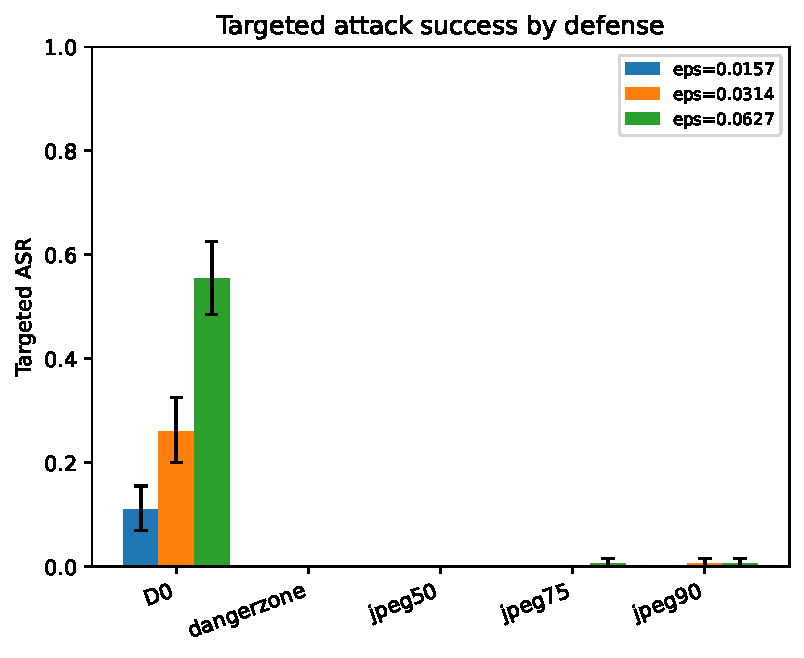
\includegraphics[width=0.78\linewidth]{figures/fig_asr_by_defense.pdf}
\caption{Targeted ASR by defense and budget (error bars: 95\% bootstrap interval).
The $\epsilon$ labels are in $[0,1]$ units: 0.0157, 0.0314 and 0.0627 are $4$, $8$ and
$16/255$.}
\label{fig:asr}
\end{figure}

Of the 185 attacks that succeeded without a defense (22, 52 and 111 at the three
budgets), Dangerzone and JPEG 50 neutralized all of them, JPEG 75 left one and JPEG 90
left two. No defense produced a success on an image where D0 failed.
Table~\ref{tab:tests} gives the paired tests at $16/255$, where the family of seven
comparisons is corrected with Holm. All four defenses differ from D0 with adjusted
$p<10^{-23}$. At $4/255$ and $8/255$ every defense also beats D0 on the exact test
(uncorrected $p\le 4.8\times10^{-7}$ at $4/255$ and $p\le 8.9\times10^{-16}$ at
$8/255$, which passes a Bonferroni threshold for twelve tests).

\begin{table}[t]
\centering
\caption{Paired comparisons at $16/255$. $(b,c)$ counts the images where only the first
or only the second condition was attacked successfully. The ASR difference is
first minus second, in percentage points, with a 95\% paired bootstrap interval.}
\label{tab:tests}
\begin{tabular}{lccc}
\toprule
Comparison & $(b,c)$ & ASR difference & Holm-adjusted $p$ \\
\midrule
Dangerzone vs D0 & (0, 111) & $-55.5$ [$-62.5$, $-48.5$] & $1.1\times10^{-24}$ \\
JPEG 50 vs D0    & (0, 111) & $-55.5$ [$-62.5$, $-48.5$] & $1.1\times10^{-24}$ \\
JPEG 75 vs D0    & (0, 110) & $-55.0$ [$-62.0$, $-48.0$] & $1.3\times10^{-24}$ \\
JPEG 90 vs D0    & (0, 110) & $-55.0$ [$-62.0$, $-48.0$] & $1.3\times10^{-24}$ \\
Dangerzone vs JPEG 50 & (0, 0) & $0.0$ [0.0, 0.0] & 1.0 \\
Dangerzone vs JPEG 75 & (0, 1) & $-0.5$ [$-1.5$, 0.0] & 1.0 \\
Dangerzone vs JPEG 90 & (0, 1) & $-0.5$ [$-1.5$, 0.0] & 1.0 \\
\bottomrule
\end{tabular}
\end{table}

\subsection{Cost to legitimate content}
Table~\ref{tab:util} gives preservation and restoration. Preservation is about 92\% for
every defense, and the intervals overlap fully: Dangerzone is at 91.5\% [87.5, 95.0],
JPEG 50 and 75 at 92.0\% and JPEG 90 at 92.5\%. Quality 90 costs as much as quality 50,
which suggests that much of the 7.5\% to 8.5\% of changed clean answers comes from the
greedy 4-bit model flipping under small input changes. We did not test that cause
directly.

Restoration shows a difference between the JPEG qualities. At $16/255$ it is 81.5\%
[76.0, 87.0] for Dangerzone, 83.0\% [77.5, 88.0] for JPEG 50, 78.5\% [72.5, 84.0] for
JPEG 75 and 68.5\% [62.0, 75.0] for JPEG 90, against 17.0\% [12.0, 22.5] with no
defense. A weak JPEG usually moves the answer away from the target without returning to
the clean answer. Dangerzone and JPEG 50 return to the clean answer more often, and
their intervals overlap.

\begin{table}[t]
\centering
\caption{Preservation (clean images, percent, 95\% interval) and restoration (attacked
images, percent) per budget.}
\label{tab:util}
\begin{tabular}{lcccc}
\toprule
 & Preservation & \multicolumn{3}{c}{Restoration} \\
\cmidrule(lr){3-5}
Defense & & $4/255$ & $8/255$ & $16/255$ \\
\midrule
D0 (none)  & 100.0 & 49.5 & 35.5 & 17.0 \\
JPEG 90    & 92.5 [88.5, 96.0] & 84.5 & 77.0 & 68.5 \\
JPEG 75    & 92.0 [88.0, 95.5] & 88.5 & 85.0 & 78.5 \\
JPEG 50    & 92.0 [88.0, 95.5] & 89.5 & 88.5 & 83.0 \\
Dangerzone & 91.5 [87.5, 95.0] & 88.0 & 87.5 & 81.5 \\
\bottomrule
\end{tabular}
\end{table}

\begin{figure}[t]
\centering
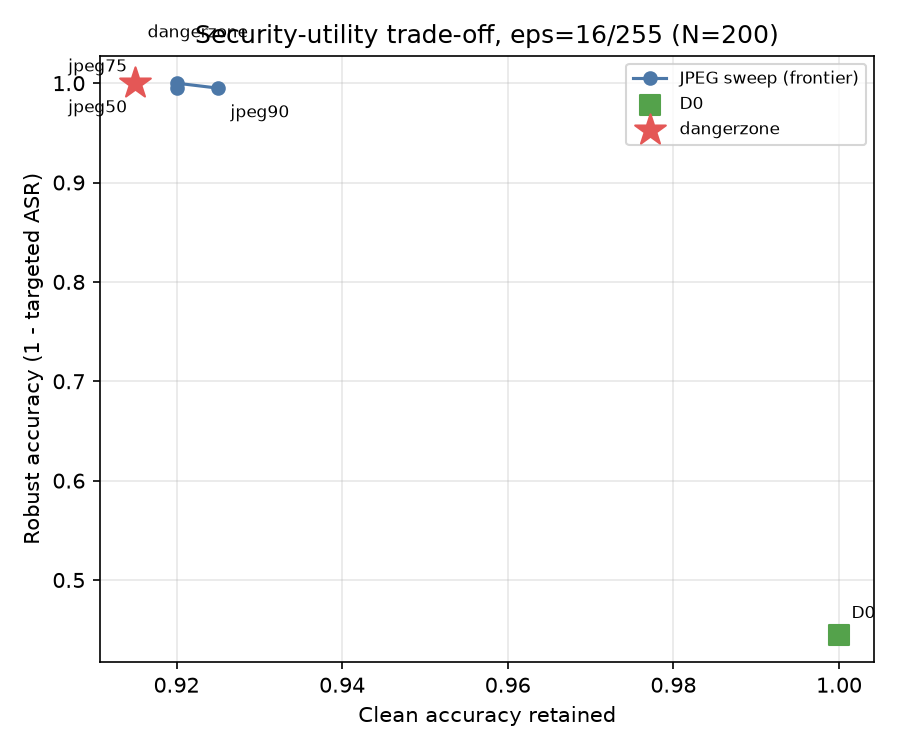
\includegraphics[width=0.62\linewidth]{figures/tradeoff_eps0.0627.png}
\caption{Security and utility at $16/255$. The vertical axis is $1-\text{ASR}$ and the
horizontal axis is preservation. The three JPEG points and Dangerzone sit in the same
corner.}
\label{fig:tradeoff}
\end{figure}

\subsection{What the defenses do to the perturbation}
Table~\ref{tab:mech} and Figure~\ref{fig:mech} show the defense-controlled residual.
Dangerzone removes the most: the residual keeps 59\% of its energy and the
high-frequency share falls from 0.82 to 0.61. JPEG 50 lowers the high-frequency share
to 0.73 but raises the residual energy by 26\%, and JPEG 75 does the same to a smaller
degree. JPEG 90 leaves the energy at 0.99 of the original and the high-frequency share
at 0.85, slightly above where it started.

\begin{table}[t]
\centering
\caption{Mean residual energy ratio and high-frequency share of the residual
$\text{defended\_adv}-\text{defended\_clean}$, over 588 attacked images per defense.
The other 12 images were processed by the pilot with an earlier metric and are
excluded.}
\label{tab:mech}
\begin{tabular}{lccc}
\toprule
Defense & Energy ratio (after / before) & High-freq. share before & after \\
\midrule
D0 (none)  & 1.00 & 0.82 & 0.82 \\
JPEG 90    & 0.99 & 0.82 & 0.85 \\
JPEG 75    & 1.14 & 0.82 & 0.80 \\
JPEG 50    & 1.26 & 0.82 & 0.73 \\
Dangerzone & 0.59 & 0.82 & 0.61 \\
\bottomrule
\end{tabular}
\end{table}

\begin{figure}[t]
\centering
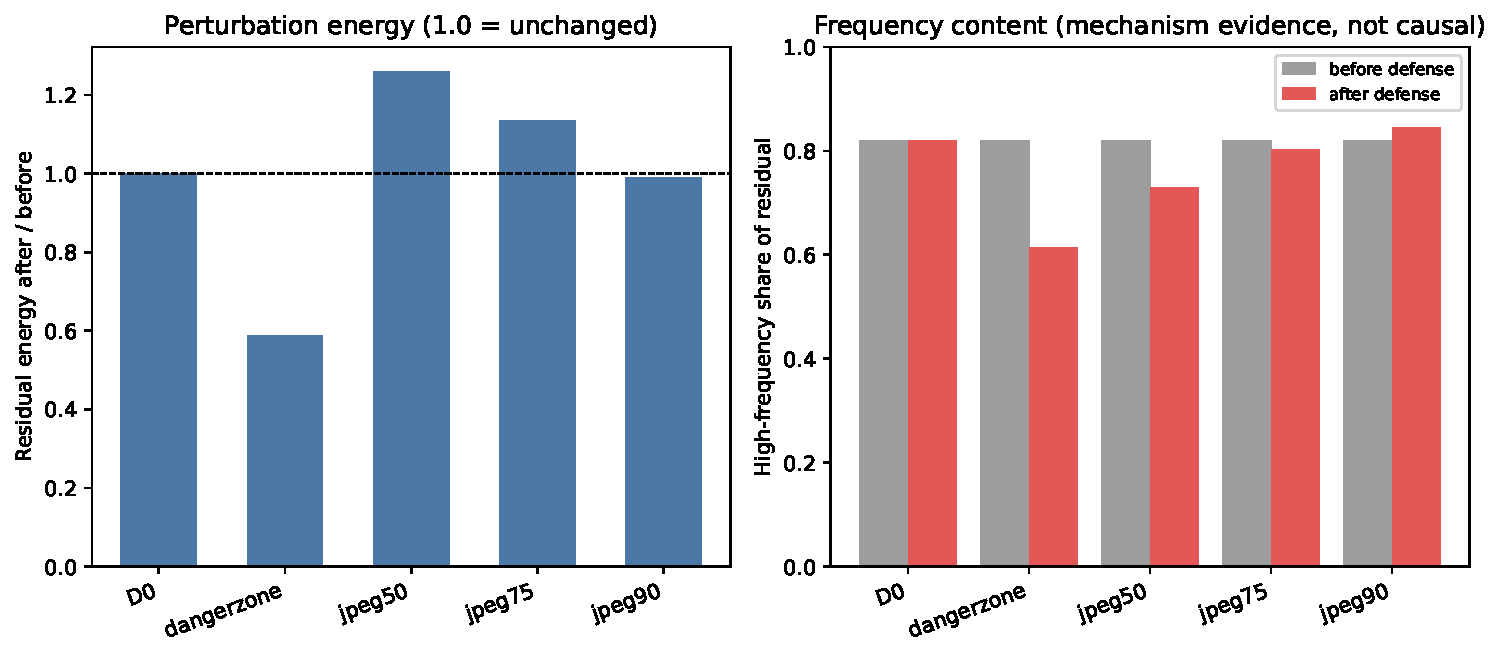
\includegraphics[width=0.95\linewidth]{figures/fig_mechanism.pdf}
\caption{Residual energy ratio (left) and high-frequency share (right) per defense.}
\label{fig:mech}
\end{figure}

% ======================================================================
\section{Discussion}
\label{sec:disc}

\textbf{RQ1: yes.} Against this attacker, every defense removes nearly all of the attack
(Table~\ref{tab:asr}). At $16/255$ the ASR falls from 55.5\% to between 0\% and 0.5\%,
and the paired tests are significant after correction.

\textbf{RQ2: no evidence that CDR beats JPEG.} Dangerzone and JPEG 50 stopped the same
attacks (zero discordant pairs), and Dangerzone against JPEG 75 and 90 differs by at
most one image of 200 (adjusted $p=1.0$). Preservation is the same within the
intervals (Figure~\ref{fig:tradeoff}), and restoration overlaps with JPEG 50. The
hypothesis that Dangerzone lies beyond the JPEG trade-off curve is not supported. A
small advantage cannot be excluded, but with ASR at the floor the test has no room to
show one. This is a limit of the attack, taken up below.

\textbf{RQ3: removal of high-frequency energy is not needed here.} Dangerzone removes
the most high-frequency energy, as expected for a render-and-rebuild pipeline. Yet JPEG
90 defeats 183 of 185 attacks while leaving the residual energy unchanged and the
high-frequency share slightly higher. A defense can break this attack without removing
the perturbation's energy. One reading is that the perturbation is tuned to the exact
pixels the model saw, and any small resampling shift breaks the optimization. We did
not test that reading, and the mechanism numbers are descriptive.

\textbf{RQ4: not tested.} The attacker never saw a defense. The finding that JPEG 90,
which changes the image least, already defeats the attack suggests that the attack is
brittle. The informative next experiment is a defense-aware
attack that approximates the defense in the backward pass or averages over its
randomness~\cite{athalye2018obfuscated,tramer2020adaptive,carlini2019evaluating}.
Without it, these results do not support the claim that CDR protects a VLM.

% ======================================================================
\section{Limitations}
\begin{itemize}
\item \textbf{One CDR tool.} Only Dangerzone, through an image-to-PDF adapter, was
measured. ICDR was blocked. The results do not speak for CDR as a category.
\item \textbf{Non-adaptive attacker and a floor effect.} With ASR near zero under every
defense, the study cannot rank the defenses against each other.
\item \textbf{Moderate attack strength.} Undefended ASR is 11\% to 55.5\%. A defense that
removes this attack has not been shown to remove a stronger one.
\item \textbf{One model, one prompt, one data set.} LLaVA-1.5-7B in 4-bit, one question,
200 images from 20 ImageNet classes at 336 px. Quantization changes both the gradients
and the answers.
\item \textbf{Model-relative metrics.} Preservation and restoration compare with the
model's own clean answer, not with ground truth.
\item \textbf{Scope.} The proposal also names typographic prompt-injection attacks.
They were not run.
\item \textbf{Statistics.} The corrected family is evaluated at $16/255$ only. The tests at
the other budgets are uncorrected exact tests computed outside the main pipeline.
Twelve images in the Dangerzone rows come from the earlier pilot, with the same images,
budget and procedure.
\item \textbf{Harm.} Success means forcing a harmless target word. No harmful content
was generated.
\end{itemize}

% ======================================================================
\section{Reproducibility}
The run directory \texttt{results/runs/full\_200} holds the configuration, environment
(Colab T4, torch 2.11, transformers 5.18), dataset manifest, per-job outputs, the
persisted adversarial arrays, \texttt{statistics.json} and the figures. The seed is 1234
throughout. The scripts, all under \texttt{scripts/}:
\begin{itemize}
\item \texttt{run\_experiment.py} runs the attacks and the JPEG conditions and resumes
by skipping finished jobs.
\item \texttt{dangerzone\_sanitize.py} and \texttt{dangerzone\_finalize.py} run the
Dangerzone condition.
\item \texttt{run\_analysis.py} and \texttt{make\_figures.py} produce every table and
figure from the stored results.
\end{itemize}
Every number in this report is read from those files.

\printbibliography

\end{document}
